\documentclass[10pt,a4paper]{article}

\usepackage[a4paper,margin=0mm]{geometry}
\usepackage[T1]{fontenc}
\usepackage[utf8]{inputenc}
\usepackage{newtxtext}
\usepackage[scaled=0.93]{helvet}
\usepackage{textcomp}
\usepackage{graphicx}
\usepackage{xcolor}
\usepackage{tikz}
\usepackage{fontawesome5}
\usepackage{hyperref}
\usepackage{enumitem}
\usepackage{ragged2e}
\usepackage{microtype}
\usetikzlibrary{calc}

\definecolor{cvteal}{RGB}{2,129,148}
\definecolor{cvbg}{RGB}{237,237,237}
\definecolor{cvtext}{RGB}{84,84,84}
\definecolor{cvlight}{RGB}{196,196,196}
\definecolor{cvorcid}{RGB}{166,206,57}

\graphicspath{{FIGURES/}}
\pagestyle{empty}
\setlength{\parindent}{0pt}
\setlength{\fboxsep}{0pt}
\pdfpagewidth=210mm
\pdfpageheight=297mm
\hypersetup{colorlinks=true,urlcolor=cvteal,linkcolor=cvteal}

\newcommand{\sans}{\fontfamily{phv}\selectfont}
\newcommand{\wide}[1]{{\sans\bfseries\textls[180]{#1}}}
\newcommand{\cvlink}[2]{\href{#1}{\textcolor{cvteal}{\underline{#2}}}}
\newcommand{\headerlink}[2]{\href{#1}{\textcolor{white}{\underline{#2}}}}

\newcommand{\headeritem}[3]{%
  {\color{white}\fontsize{9.3}{10.5}\selectfont
  \faIcon{#1}\hspace{1.2mm}#3}%
}

\newcommand{\sideheading}[1]{%
  \vspace{0.65mm}%
  \noindent
  
\begin{tikzpicture}[x=1mm,y=1mm,baseline=-1.6mm]
    \fill[cvteal] (0,0) -- (7,3.6) -- (0,7.2) -- (2.4,3.6) -- cycle;
  \end{tikzpicture}%
  \hspace{2mm}{\sans\bfseries\fontsize{14.5}{15.5}\selectfont #1}\par
  \vspace{0.65mm}%
}

\newcommand{\skillgroup}[2]{%
  \vspace{0.35mm}
  {\centering{\sans\bfseries\fontsize{12.5}{13.2}\selectfont\color{cvteal}#1}\par}
  \vspace{0.35mm}
  {\fontsize{8.9}{11.2}\selectfont #2\par}
}

\newcommand{\langbar}[3]{%
  \vspace{0.35mm}
  {\fontsize{10.2}{11.0}\selectfont #1\par}
  \begin{tikzpicture}[x=1mm,y=1mm]
    \fill[cvlight,rounded corners=0.65mm] (0,0) rectangle (45.5,1.65);
    \fill[cvteal,rounded corners=0.65mm] (0,0) rectangle (#3,1.65);
  \end{tikzpicture}%
  \hfill{\fontsize{10.4}{11.0}\selectfont #2}\par
}

\newcommand{\pubicon}{%
  
\begin{tikzpicture}[x=1mm,y=1mm]
    \fill[cvteal,rounded corners=1.1mm] (0,0) rectangle (5.8,9.2);
    \node[text=cvorcid,font=\fontsize{6.8}{6.8}\selectfont] at (2.9,4.6) {\faIcon{link}};
  \end{tikzpicture}%
}

\newcommand{\orcidicon}{%
  
\begin{tikzpicture}[x=1mm,y=1mm,baseline=-2.4mm]
    \fill[cvorcid] (2.9,2.9) circle (2.9);
    \node[text=white,font=\sans\bfseries\fontsize{5.2}{5.2}\selectfont] at (2.9,2.9) {iD};
  \end{tikzpicture}%
}

\newcommand{\publication}[2]{%
  \noindent
  \begin{minipage}[t]{7mm}\vspace{0pt}#1\end{minipage}%
  \hspace{1.1mm}%
  \begin{minipage}[t]{44.5mm}\vspace{0pt}\fontsize{7.85}{9.05}\selectfont #2\end{minipage}%
  \par\vspace{0.18mm}
}

\newcommand{\mainsection}[1]{%
  \vspace{0.2mm}
  \noindent\makebox[\linewidth][c]{%
    \textcolor{cvteal}{\rule{0.25\linewidth}{0.65pt}}%
    \hspace{2.1mm}{\color{cvteal}\wide{\fontsize{17.2}{18}\selectfont #1}}%
    \hspace{2.1mm}\textcolor{cvteal}{\rule{0.25\linewidth}{0.65pt}}%
  }\par\vspace{2.0mm}
}

\newcommand{\entry}[5]{%
  \noindent
  {\fontsize{12.4}{13.4}\selectfont\bfseries #1}%
  \hfill{\fontsize{11.0}{12.0}\selectfont #2}\par
  \vspace{0.7mm}
  {\fontsize{11.0}{12.0}\selectfont #3\textcolor{cvtext}{\ - #4}}\par
  \vspace{0.8mm}
  {\color{cvtext}\fontsize{9.85}{11.95}\selectfont\justifying #5\par}
}

\newcommand{\divider}{%
  \vspace{1.5mm}\noindent\textcolor{cvteal}{\rule{\linewidth}{0.55pt}}\par\vspace{1.5mm}
}

\newcommand{\cvitems}{%
  \begin{itemize}[leftmargin=5.5mm,itemsep=0.35mm,topsep=0.6mm,parsep=0pt]
}
\newcommand{\cvitemsend}{\end{itemize}}

\newcommand{\awardentry}[3]{%
  \noindent{\fontsize{11.0}{12.0}\selectfont #1}%
  \hfill{\fontsize{11.0}{12.0}\selectfont #2}\par
  \vspace{0.8mm}
  {\color{cvtext}\fontsize{9.85}{11.95}\selectfont\justifying #3\par}
}

\begin{document}
\null
\begin{tikzpicture}[remember picture,overlay,x=1mm,y=-1mm]
\begin{scope}[shift={(current page.north west)}]
  \fill[cvteal] (0,0) rectangle (210,36.1);
  \fill[cvbg] (0,36.1) rectangle (210,297);

  \draw[cvteal,line width=1.05mm,rounded corners=5mm]
    (0.5,39.2) -- (53.4,39.2) -- (60.1,45.9) -- (60.1,287.7) -- (53.4,294.2) -- (3.0,294.2);

  \begin{scope}
    \clip[rounded corners=4.2mm] (3.0,2.8) rectangle (60.0,29.9);
    \node[inner sep=0pt] at (31.5,16.35) {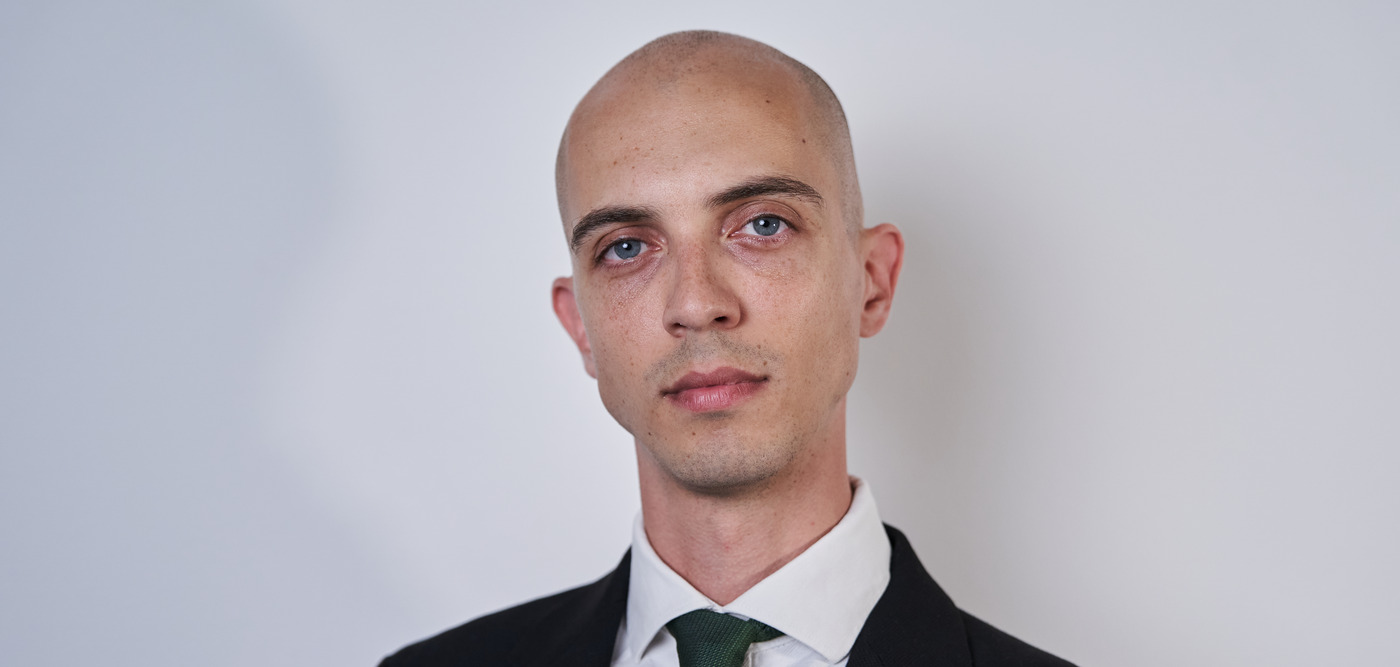
\includegraphics[width=57.0mm]{CV_picture_header.jpg}};
  \end{scope}

  \node[anchor=north,text=white,font=\sans\bfseries\fontsize{31}{33}\selectfont] at (135,2.8) {Fabio Vulpi};
  \node[anchor=north,text=white,font=\sans\bfseries\fontsize{14.6}{15.5}\selectfont] at (135,14.8) {Ph.D. in Mechanical Engineering and Management};

  \node[anchor=west] at (63.5,23.0) {\headeritem{phone}{tel:+393803485030}{+39 3803485030}};
  \node[anchor=west] at (121.0,23.0) {\headeritem{map-marker-alt}{}{70124, Bari (BA), Italy}};
  \node[anchor=west] at (189.0,23.0) {\headeritem{calendar-alt}{}{21/12/1995}};
  \node[anchor=west] at (63.5,30.0) {\headeritem{linkedin}{https://linkedin.com/in/fabio-vulpi}{\headerlink{https://linkedin.com/in/fabio-vulpi}{linkedin.com/in/fabio-vulpi}}};
  \node[anchor=west] at (121.0,30.0) {\headeritem{github}{https://github.com/vulpi-f}{\headerlink{https://github.com/vulpi-f}{github.com/vulpi-f}}};
  \node[anchor=west] at (169.8,30.0) {\headeritem{envelope}{mailto:vulpi.fabio@gmail.com}{vulpi.fabio@gmail.com}};

  \node[anchor=north west,inner sep=0pt] at (3.0,39.2) {%
    \begin{minipage}[t]{53.6mm}
      \sideheading{ABOUT ME}
      {\fontsize{9.85}{12.05}\selectfont
      Daring and versatile, I firmly believe that attaining successful outcomes relies on both the ability to ask pertinent questions and the commitment to finding the answers.\par}

      \sideheading{SOFT-SKILLS}
      {\fontsize{9.9}{11.1}\selectfont
      \begin{itemize}[leftmargin=5.2mm,itemsep=0.15mm,topsep=0mm,parsep=0pt]
        \item Pragmatic
        \item Team working
        \item Result Oriented
      \end{itemize}}

      \sideheading{DIGITAL SKILLS}
      \skillgroup{Physic Simulation}{%
        \begin{tabular}{@{}l@{\hspace{2.1mm}\vrule\hspace{2.1mm}}l@{}}
          MATLAB & Ansys FLUENT\\
          Simulink & Wolfram Mathematica
        \end{tabular}}
      \skillgroup{\textmu C programming}{%
        \begin{tabular}{@{}l@{\hspace{2.1mm}\vrule\hspace{2.1mm}}l@{\hspace{2.1mm}\vrule\hspace{2.1mm}}l@{\hspace{2.1mm}\vrule\hspace{2.1mm}}l@{}}
          Debian & Python & C & Arduino\\
          Linux & ROS & C++ & C\#
        \end{tabular}}
      \skillgroup{3-D Modeling}{%
        \begin{tabular}{@{}l@{\hspace{2.1mm}\vrule\hspace{2.1mm}}l@{}}
          AutoCAD 2D & Autodesk Invetor\\
          SolidWorks & Cura (Ultimaker)\\
          MeshLab & Eagle - PCB design
        \end{tabular}}

      \sideheading{LANGUAGES}
      \langbar{Italiano}{C 2}{45.5}
      \langbar{English}{C 1}{38.0}
      \langbar{Deutsch}{A 2}{15.0}

      \sideheading{PUBLICATIONS}
      \publication{\orcidicon}{Kalman Supervised Network for improved Model Predictions.}
      \publication{\pubicon}{Recurrent and convolutional NN for deep terrain classification by autonomous robots.}
      \publication{\pubicon}{An RGB-D multi-view perspective for autonomous agricultural robots.}
      \publication{\pubicon}{On the role of feature and signal selection for terrain learning in planetary exploration.}
      \publication{\pubicon}{Usability Study of WISE for Movement Assessment and Exercise.}
      \publication{\pubicon}{Wearable Inertial Sensors for Range of Motion Assessment (WISE).}
    \end{minipage}};

  \node[anchor=north west,inner sep=0pt] at (63.4,38.8) {%
    \begin{minipage}[t]{143.8mm}
      \mainsection{WORK EXPERIENCE}
      \entry{Experienced Consultant}{10/2024 - current}
        {\cvlink{https://www.amaris.com/}{Amaris Consulting}}
        {Turin (IT)}
        {Vehicle Functional Safety (FuSa) consultant for ISO 26262:2018. Partnered with the FuSa Manager on the Safety Concept and Development Interface Agreement (DIA), led Hazard Analysis and Risk Assessment (HARA) and Failure Modes and Effects Analysis (FMEA) reviews. Validated ISO-compliant safety requirements throughout the automotive safety lifecycle.}
      \divider
      \entry{Software System Engineer}{01/2023 - 10/2024}
        {\cvlink{https://www.bosch.it/}{Bosch CVIT}}
        {Bari (IT)}
        {Served as a Functional Safety Software Engineer on the top-level V-model for Engine and Battery Control Unit development--ensuring ISO 26262 compliance across light-duty and heavy-duty platforms, diesel and electric powertrains. Engineered AI and ML driven vehicle convenience features (such as passive keyless entry and gesture-based trunk release) leveraging advanced signal processing and device-tracking models.}
      \divider
      \entry{Software Automation Engineer}{11/2022 - 01/2023}
        {\cvlink{https://www.linksmt.it/}{Links Management \& Technology}}
        {Bari (IT)}
        {Engineered Artificial Intelligence and Machine Learning software solutions to optimize automation workflows.}

      \mainsection{EDUCATION}
      \entry{Ph.D. in Mechanical Engineering and Management}{11/2019 - 04/2023}
        {\cvlink{https://www.poliba.it/}{Polytechnic of Bari}}
        {Bari (IT)}
        {Collaborated with \cvlink{https://www.stiima.cnr.it/}{CNR-STIIMA} on EU-funded projects \cvlink{https://www.ade-project.eu/}{ADE}, \cvlink{https://www.atlas-h2020.eu/}{ATLAS}, and \cvlink{https://antonio-project.eu/}{ANTONIO}, leading HW/SW development and AI/ML algorithm design for mechanical systems.
        \cvitems
          \item ADE: Implemented deep-learning terrain-classification pipelines for autonomous exploration rovers.
          \item ATLAS: Engineered a ROS-based, multi-sensor robotic platform for 3D reconstruction and analysis of agricultural fields.
          \item ANTONIO: Developed advanced signal- and image-processing workflows for crop-monitoring automated guided robots (AGRs).
        \cvitemsend}
      \divider
      \entry{Master of Science in Mechanical Engineering}{10/2017 - 10/2019}
        {\cvlink{https://www.nyu.edu/}{NYU}}
        {New York (USA)\hfill 110L/110 - GPA 3.952/4}
        {Completed a double-degree program in Mechanical Engineering, specializing in Mechatronics and Robotics, in collaboration with the Polytechnic of Bari. Authored an M.S. thesis in Medical Engineering field on wearable inertial-sensor systems for quantitative assessment of upper-extremity range of motion.}
      \divider
      \entry{Bachelor Degree in Mechanical Engineering}{07/2014 - 07/2017}
        {\cvlink{https://www.poliba.it/}{Polytechnic of Bari}}
        {Bari (IT)\hfill 109/110}
        {Performed physics-based modeling and numerical computation to investigate the nonlinear dynamics of oscillators with a bistable potential.}

      \mainsection{AWARDS}
      \awardentry{\cvlink{https://www.ingeniarius.pt/}{Ingeniarius Ltd}\textcolor{cvtext}{\ - Porto (PT)}}{RobotCraft First Place Award - 08/2022}
        {The competition challenged me to design and assemble an autonomous mobile robot that would fully explore a maze and generate LiDAR-based SLAM maps in ROS, then re-navigate the maze optimizing the path using its computed map. I developed real-time C++ and Python algorithms for mapping and path planning and integrated Arduino-driven motor control.}
    \end{minipage}};
\end{scope}
\end{tikzpicture}
\end{document}
